\subsection{Equivalent capacitance and inductance}

The equivalent capacitance and equivalent inductance are given by equations \ref{eq:equiv_capacitance} and \ref{eq:equiv_inductance}, respectively.

\begin{equation}
C_{\rm equ} \approx \frac{2 k_{\rm z}^{\rm (10)} b}{\pi^2 f W_{\rm 10}^{\rm TE}} \ln \left[ \csc \left( \frac{\pi s}{2a} \right) \right]
\label{eq:equiv_capacitance}
\end{equation}

\begin{equation}
L_{\rm equ} \approx \frac{a \mu_{\rm r} \mu_{\rm 0}}{2 \pi \cot^2 \left( \frac{\pi s}{2a} \left[ 1 + \csc^2 \left( \frac{\pi s}{2a}\right) \right] \right)}
\label{eq:equiv_inductance}
\end{equation}

The equivalent capacitance is plotted in figure \ref{fig:equiv_capa}.

\begin{figure}[h t b p]
	\centering
	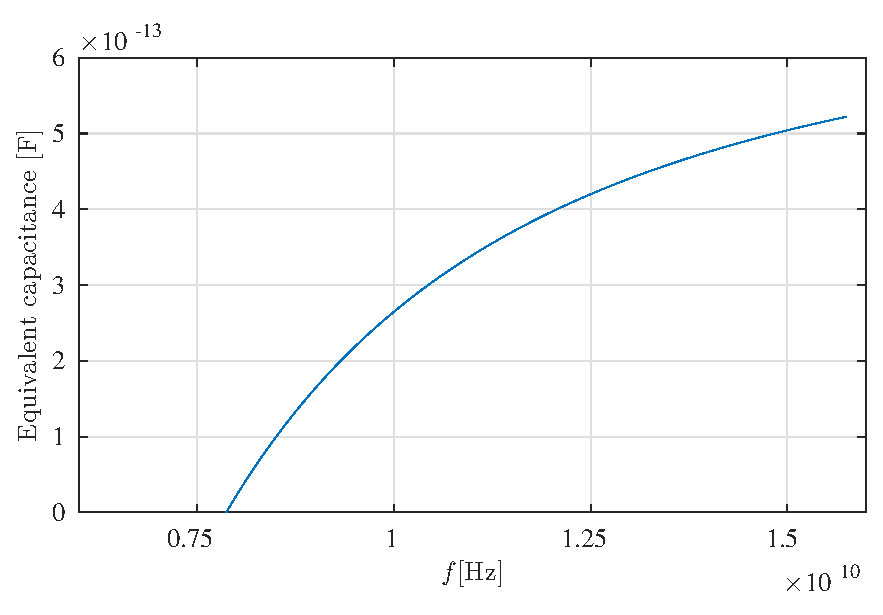
\includegraphics[width=\textwidth,keepaspectratio]{figures/equiv_capacitance.eps}
	\caption{Equivalent capacitance over the unimodal frequency band.}
	\label{fig:equiv_capa}
\end{figure}

The equivalent inductance does not vary with frequency.
For the specified waveguide, $L_{\rm equ} \approx \SI{2.1633e-8}{\henry\slash\meter}$.